\documentclass{beamer}
\usepackage{graphicx,mathtools,amssymb,amsthm}
\usepackage[thaifont=TH Sarabun New]{thaispec}
\usetheme{Madrid}
\usecolortheme{wolverine}

\title{แบบจำลองทางคณิตศาสตร์การขายครัวซองค์}
\author{จัดทำโดย \\
	นายอภิชาติ ทิพยโอสถ 116510901020-7 \\
	นางสาวอนาตี มะหะหมัด 116510901022-3 \\
	นางสาวอจิรวดี จันทวรรณ 116510901026-4}

\date{1 มีนาคม 2567}

\begin{document}

\begin{frame}
\maketitle
\end{frame}

\begin{frame}
\frametitle{บทคัดย่อ (Abstract)}
แบบจำลองทางคณิตศาสตร์การทำร้านครัวซองค์ เป็นแบบจําลองที่ถูกสร้างขึ้นเพื่อวิเคราะห์และวางแผนในการลงทุนรวมถึงกลยุทธ์ทางการเงินต่างๆ โดยการคํานวณต้นทุนในการทําครัวซองค์เพื่อให้ถูกขายออกให้หมดและไม่ขาดทุนในแต่ละครั้ง และยังสามารถคาดการณ์ถึงอนาคตว่าจะได้กำไรเมื่อขายในเดือนที่เท่าไหร่
\end{frame}

\begin{frame}
\frametitle{ความรู้พื้นฐานที่จำเป็น (Basic Knowledge)}
\begin{columns}
\column{0.5\textwidth}
\begin{figure}[h!]
\includegraphics[scale=0.1]{C1.jpg}
\centering
\end{figure}
\column{0.5\textwidth}
มีที่มาจริงๆจากสงครามระหว่างจักรวรรดิออตโตมันและกรุงเวียนนาประเทศออสเตรียโดยมีความรุนแรงถึงขั้นปิดล้อมกรุงเวียนนาเลยทีเดียวแต่สุดท้ายชาวเวียนนาก็สามารถเอาชนะสงครามครั้งนี้ได้ และเพื่อเป็นการเฉลิมฉลองชัยชนะครั้งนี้ ชาวเวียนนาจึงได้ริเริ่มอบขนมปังที่มีลักษณะคล้ายรูปพระจันทร์ครึ่งเสี้ยวซึ่งก็นํามาจากสัญลักษณ์บนธงของประเทศของศัตรูและใช้ชื่อเรียกว่าขนมคิปเฟล (Kipferl)นั่นเอง
\end{columns}
\end{frame}

\begin{frame}
\frametitle{ความรู้พื้นฐานที่จำเป็น (Basic Knowledge)}
การคำนวณค่าใช้จ่ายและราคาขาย 
การมีสูตรทำให้การทำงานของเราเป็นระบบมากขึ้น สามารถทำบัญชีรายรับ รายจ่าย และสามารถรู้ต้นทุนของสินค้า และวิธีคำนวนต้นทุน จะสามารถราคาขายให้เหมาะสมกับสินค้าของเรา การคิดต้นทุนเป็นสิ่งสำคัญมากในการทำธุรกิจ ควรนำราคาต้นทุนของวัตถุดิบ มาคำนวณรวมกับค่าใช้จ่ายอื่นๆของทางร้าน เพื่อให้มองเห็นภาพรวมทั้งหมดเพราะหากคำนวนไม่ถูกก็ไม่สามารถกำหนดราคาขายได้
\end{frame}

\begin{frame}
\frametitle{โจทย์ (Proposition)}
\begin{columns}
\column{0.5\textwidth}
นางสาวเอต้องการลงทุนกับธุรกิจร้านทำครัวซองค์ ต้องการหารายได้จากการขายครัวซองค์ จงนําเสนอแบบจําลองทางคณิตศาสตร์เพื่อหาคําตอบว่านางสาวเอต้องขายครัวซองค์เป็นระยะเวลากี่เดือนถึงจะเริ่มได้กําไร
\column{0.5\textwidth}
\begin{figure}[h!]
\includegraphics[scale=0.1]{E1.jpg}
\centering
\end{figure}
\end{columns}
\end{frame}

\begin{frame}
\frametitle{ปัญหา (Questions)}
ต้องการแบบจำลองทางคณิตศาสตร์ที่ตอบปัญหาดังนี้
\begin{itemize}
    \item[-] การลงทุนธุรกิจร้านครัวซองค์ ใช้ระยะเวลากี่เดือนถึงจะได้กำไร
	\item[-] ต้องจำหน่ายออกให้ได้ทุกวัน
\end{itemize}
\end{frame}

\begin{frame}
\frametitle{องค์ประกอบ (Factors)}
\begin{center}
\begin{table}[!ht]
\centering
\begin{tabular}{ |c|c|c|c| }
\hline
\textbf{สัญลักษณ์ } & \textbf{ประเภท } & \textbf{ตัวแปร } & \textbf{หน่วย } \\
\hline
$N$ & พารามิเตอร์ & ยอดขาย & บาท/เดือน \\
\hline
$P$ & ตัวแปรผลลัพธ์ & กําไร(เดือน) & บาท/เดือน \\
\hline
$T$ & ตัวแปรนำเข้า & ระยะเวลาลงทุน & เดือน \\
\hline
$X$ & พารามิเตอร์ & ค่าต้นทุนต่อเดือน & บาท/เดือน \\
\hline
$Y$ & พารามิเตอร์ & ค่าต้นทุนสินค้า & บาท/เดือน \\
\hline
$Z$ & พารามิเตอร์ & ค่าต้นทุนการตลาด & บาท/เดือน \\
\hline
$C$ & พารามิเตอร์ & ราคาขายครัวซองค์ & บาท/เดือน \\
\hline
$J$ & พารามิเตอร์ & จํานวนครัวซองค์ & ชิ้น \\
\hline
\end{tabular}
\caption{ตารางแสดงองค์ประกอบ}
\label{table : 1}
\end{table}
\end{center}
\end{frame}

\begin{frame}
\frametitle{แผนภาพแสดง Model อย่างง่าย}
\begin{figure}[!ht]
	\centering
	\includegraphics[scale=0.12]{ice16.jpg}
	\caption{ภาพแสดงตัวแปรในโจทย์}
	\label{fig : graph2}
\end{figure}
\end{frame}

\begin{frame}
\frametitle{สมมติฐาน (Assumptions)}
\begin{itemize}
	\item[-] แบบจําลองนี้สามารถให้คําตอบได้ว่าจะต้องขายกี่ชิ้นถึงจะได้กําไรและภายในระยะเวลากี่เดือน
	\item[-] ในการขายในแต่ละเดือนรายได้จะต้องไม่ติดลบ
\end{itemize}
\end{frame}

\begin{frame}
\frametitle{ปัญหาทางคณิตศาสตร์ (Mathematical Problem)}
จากปัญหาและสัญลักษณ์ข้างต้น สามารถเขียนปัญหาได้ในรูปแบบของคณิตศาสตร์ได้ดังนี้ \par
กำหนดให้ ${N,P,T,X,Y,Z,C,J}\in\mathbb{N}$ จงหา ${T}\in\mathbb{R_{+}}$ 
ที่ทำให้ $P>0$
\end{frame}

\begin{frame}
\frametitle{สมการและผลเฉลย (Equations and Deuteronomy)}
\begin{equation}
	P = (N - Y - Z)T - X > 0 
\end{equation}
\begin{align}
	N = (C)\cdot (J)
\end{align}
\textbf{Solution} เราจะได้กำไรเมื่อ
\begin{align}
	(N-Y-Z)T-X>0 \\
	(N-Y-Z)T>x \\
	T>\frac{X}{N-Y-Z} 
\end{align}
\end{frame}

\begin{frame}
\frametitle{ผลลัพธ์เชิงตัวเลข (Numerical results)}
หลังจากการสืบค้นรวบรวมข้อมูลจริงแล้วนั้น สามารถคาดเดารายได้และต้นทุนได้ดังกรณี
ตัวอย่างดังต่อไปนี้
\section{การหาระยะเวลาการขายกี่เดือนถึงจะได้กำไร}
ราคาโดยเฉลี่ยต่อลูกค้า 1 คน$(C)$ 70 บาทต่อคน \\
จำนวนชิ้นที่ขาย$(J)$ โดยประมาณ 60ชิ้นต่อวัน หรือ 1,800 ชิ้นต่อเดือน \\
จากสมการที่ (3.1)\par 
\begin{equation}
	P = 450,000-((70)(1,800) - 10,000 - 2,500)T > 0  
\end{equation}
จากสมการที่ (3.4) จะได้ผลเฉลยคือ
\begin{align*}
T &> \frac{450,000}{(70)(1,800) - 10,0000 - 2,500} \\
T &> \frac{450,000}{113,500} \\
T &> 4 \\
\end{align*}
\end{frame}

\begin{frame}
\frametitle{ผลลัพธ์เชิงตัวเลข (Numerical results)}
จะได้ว่าถ้าใน 1 วัน นางสาวเอขายได้วันละ$(J)$ 60 ชิ้น จะทำให้การลงทุนในการขายครัวซองค์นี้ ใช้ระยะ
เวลาประมาณ 4 เดือน ถึงจะเริ่มได้กำไร
\end{frame}

\begin{frame}
\frametitle{โปรแกรมที่ใช้ในการคำนวณ}
\begin{figure}[h!]
\includegraphics[scale=0.50]{B2.jpg}
\centering
\end{figure}
\end{frame}

\begin{frame}
\frametitle{โปรแกรมที่ใช้ในการคำนวณ}
\begin{figure}[h!]
\includegraphics[scale=0.50]{B3.jpg}
\centering
\end{figure}
\end{frame}

\begin{frame}
\frametitle{โปรแกรมที่ใช้ในการคำนวณ}
\begin{figure}[h!]
\includegraphics[scale=0.40]{B4.jpg}
\centering
\end{figure}
\end{frame}

\begin{frame}
\frametitle{บทวิเคราะห์}
\textbf{ปัญหา:}การลงทุนธุรกิจร้านขายครัวซองค์  ใช้ระยะเวลากี่เดือนถึงจะได้กำไร\\
	ในการลงทุนในธุรกิจร้านครัวซองค์นี้ ถ้ามีลูกค้าในแต่ละวัน 60 คน หรือต่อเดือน 1,800 คน จะทําให้การลงทุนในธุรกิจนี้ ใช้ระยะเวลาประมาณ 4 เดือน ถึงจะเริ่มได้กำไร
\begin{figure}[h!]
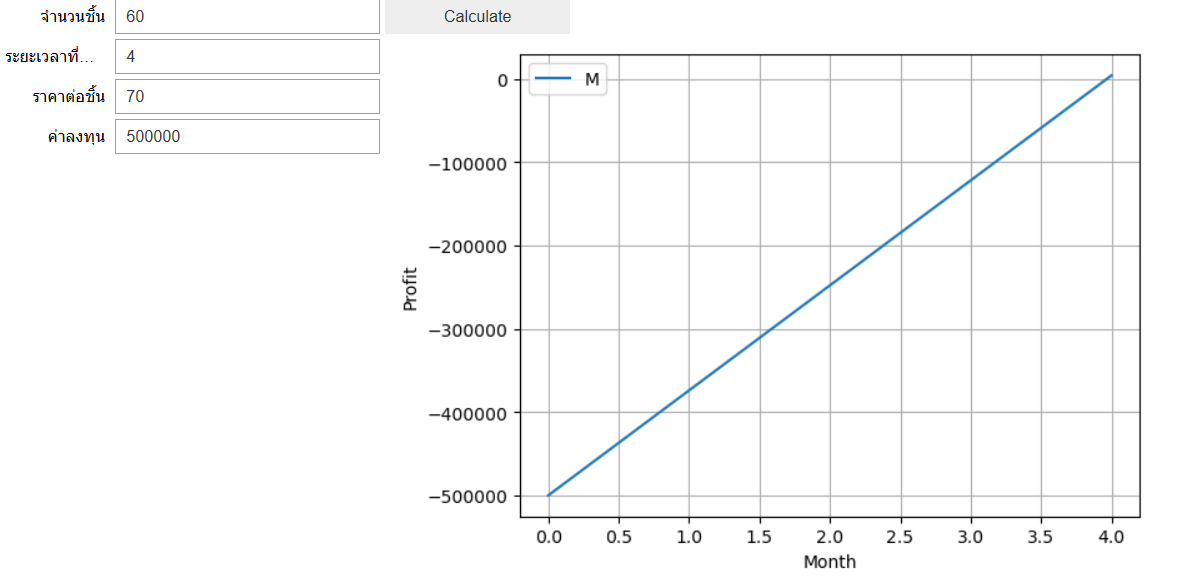
\includegraphics[scale=0.40]{B1.jpg}
\centering
\end{figure}
\end{frame}

\begin{frame}
\frametitle{สรุป (Summarize)}
จากการที่ได้ทำแบบจำลองทางคณิตศาสตร์ในการที่จะเริ่มลงทุนกับธุรกิจการขายครัวซองค์ เราจำเป็นต้องคำนึงถึงเงินลงทุนที่มีอยู่อย่างจำกัดเป็นหลักและต้องคำนึงถึงค่าสินค้าต่างๆ มีการสำรองค่าใช้จ่ายต่างๆเผื่อสำหรับกรณีฉุกเฉิน
ถ้าคุณมีเงินมากพอคุณก็สามารถเปิดร้านขายครัวซองค์ได้ และสามารถทำให้ได้กำไรโดยภายในปีนั้นได้
สิ่งที่ผู้จัดทำต้องการ คือการคำนวณผลกำไรในแต่ละเดือน และในแต่ละเดือนรายได้จะต้องไม่ติดลบ
สุดท้ายนี้ แบบจำลองทางคณิตศาสตร์ธุรกิจการขายครัวซองต์ ก็เป็นเพียงแบบจำลองตัวอย่างที่ใช้ประกอบการตัดสินใจในการลงทุนเท่านั้น ทั้งนี้อยู่ที่ความเห็นและความเหมาะสมของผู้ลงทุนแต่ละคนว่าจะลงทุนในธุรกิจนี้หรือไม่ เพราะการลงทุนมีความเสี่ยงควรศึกษาเพิ่มเติมให้มาก ก่อนจะ ดำเนินธุรกิจต่างๆไม่ว่าจะเป็นอะไรก็ตาม
\end{frame}


\end{document}
